\documentclass[student, noshadow, lsr, english, aspectratio=169, t]{ITR_LSR_slides}

\setbeamertemplate{frametitle}{%
  \vspace{0.3cm}% Space between top edge and title
  \if@center
    \begin{centering}
      \textbf{\vphantom{Sp}\insertframetitle\vphantom{Sp}}
      \par
    \end{centering}
  \else
    \textbf{\vphantom{Sp}\insertframetitle\vphantom{Sp}}
    \par
  \fi
  \vspace{0.3cm}% Space between title and content
}

% Add top margin to frames without titles
\addtobeamertemplate{frame begin}{%
  \ifx\insertframetitle\@empty
    \vspace{0.8cm}% Space at top of frames without titles
  \fi
}{}

\addbibresource{ref.bib}
\graphicspath{{pics/}{logos/}}

\title{Analysis and Control of Time-Varying and Perturbed Systems}
\presenter{Keno Bürger}
\typeofpres{Advanced Nonlinear Control}

\usepackage{multirow}
\usepackage{graphicx}
\usepackage[T1]{fontenc}
\usepackage{lmodern}
\usepackage{tabularx}
\usepackage{enumitem}
\usepackage{adjustbox}
\usepackage{booktabs}
\usepackage{makecell}
\PassOptionsToPackage{most}{tcolorbox}
\usepackage{tcolorbox}
\usepackage{amsmath,amssymb}
\usepackage{amsmath,amssymb}
\usepackage{hyperref}

% Load hyperref as the last package before document begins
\hypersetup{
	pdftitle={Advanced Nonlinear Control: Lyapunov Stability and Perturbations},
	pdfauthor={Keno Bürger},
	pdfsubject={Nonlinear Control Theory},
	pdfkeywords={Lyapunov stability, exponential stability, boundedness, ultimate boundedness, perturbations, nonlinear control},
	pdfcreator={LaTeX with Beamer},
    pdfproducer={pdfTeX},
}

% Fix for potential BOM or invisible characters
\pdfstringdefDisableCommands{%
  \def\translate#1{#1}%
}

\begin{document}

\begin{frame}
    \titlepage
\end{frame}


%%%%%%%%%%%%%%%%%%%%%%%%%%%%%%%%%%%%%%%%%%%%%%%%%%%%%%
\section{Motivation}

\begin{frame}{Why Study Time-Varying Perturbed Systems?}
	\begin{itemize}
		\item \textbf{Real-World Imperfections:}
		\begin{itemize}
			\item Systems rarely time-invariant
			\item Parameters drift, components age, environment shifts
			\item \textit{Ex:} Aircraft dynamics change with fuel, altitude, air density
		\end{itemize}
		\item \textbf{Uncertainty Omnipresent:}
		\begin{itemize}
			\item External disturbances (wind gusts, load variations)
			\item Internal uncertainties (sensor noise, actuator inaccuracies, unmodeled dynamics)
			\item \textit{Ex:} Robot arm payload
		\end{itemize}
		\item \textbf{Performance \& Robustness Demands:}
		\begin{itemize}
			\item Modern control needs high performance (precision, speed) and robust stability
			\item Ignoring variations $\rightarrow$ poor performance, instability, failure
		\end{itemize}
	\end{itemize}
\end{frame}

\begin{frame}
    \frametitle{Understanding Perturbation Types}

    % \textbf{Motivation:} Real-world systems exhibit time-dependence, modeling errors, external disturbances

    % \vspace{0.5cm}
    \textbf{General System Form:}
    \[\dot{\underline{x}} = f(\underline{x}) + g(\underline{x}, t)\]

	\vspace{-0.5em}
    \begin{columns}[t,totalwidth=\textwidth]
        \column{0.48\textwidth}
		\begin{tcolorbox}[title=Vanishing Perturbation:]
			% \textbf{Vanishing Perturbation:}
			\begin{itemize}
				\item $g(\underline{x}, t) \to 0$ as $\underline{x} \to 0$
				\item Preserves exponential stability
				\item Examples: modeling errors, unmodeled dynamics
			\end{itemize}
		\end{tcolorbox}

        \column{0.48\textwidth}
        \begin{tcolorbox}[title=Non-Vanishing Perturbation:]
			\begin{itemize}
				\item $g(\underline{x}, t) \not\to 0$ as $\underline{x} \to 0$
				\item Leads to ultimate boundedness
				\item Examples: constant disturbances, sensor noise
			\end{itemize}
		\end{tcolorbox}
    \end{columns}
\end{frame}

% \begin{frame}
%     \frametitle{Main Objective}

%     \textbf{Based on:}
%     \begin{itemize}
%         \item \textit{Nonlinear Control} (Ch. 4): Time-varying and perturbed systems
%         \item \textit{Nonlinear Systems} (Ch. 9, 11.5): Stability under perturbations
%     \end{itemize}
% 	\vspace{0.5cm}
%     \textbf{Objective:}
%     \begin{itemize}
% 		\item Formulate practical and broadly applicable stability conditions
%         \item Analyze stability under \textbf{vanishing perturbations} using comparison functions
%         \item Study ultimate boundedness for systems with \textbf{non-vanishing perturbations}
%         % \item Apply Lyapunov-based methods for robust analysis of nonlinear, time-varying systems
%     \end{itemize}
% \end{frame}

%%%%%%%%%%%%%%%%%%%%%%%%%%%%%%%%%%%%%%%%%%%%%%%%%%%%%%
\section{Prerequisites}

\begin{frame}
	\frametitle{Lyapunov Theory for Time-Varying Systems}
	% \begin{itemize}
	% 	\item Definition of Uniform, Asymptotic and exponential stability \cite{muennighoff_s1_2025}
	% 	\item Application of Lyapunov Stability Theorems
	% \end{itemize}
	\textbf{Assumptions:}
	\begin{itemize}
		\item Origin $\underline{x}=0$ is an equilibrium point
		\item Lyapunov function $V(t,\underline{x})$ is continuously differentiable, positive definite and radially unbounded
		\item Derivative of Lyapunov function is negative definite
	\end{itemize}
	\vspace{0.2cm}
	\begin{tcolorbox}[title=Globally uniformly exponentially stable:]
		\vspace{-0.4cm}
		\begin{align*}
			\exists\, c_i, \alpha > 0: & \; c_1\left\|\underline{x}\right\|^\alpha \leq V(t,\underline{x}) \leq c_2\left\|\underline{x}\right\|^\alpha  \\
			& \dot{V}(t,\underline{x}) \leq -c_3\|\underline{x}\|^\alpha
		\end{align*}	
	\end{tcolorbox}
	
\end{frame}

\begin{frame}
	\frametitle{Boundedness and Ultimate Boundedness}
	% \begin{itemize}
	% 	\item Differences
	% 	\item Build bridge to non vanishing and vanishing perturbations
	% \end{itemize}
	\begin{figure}
		\centering
		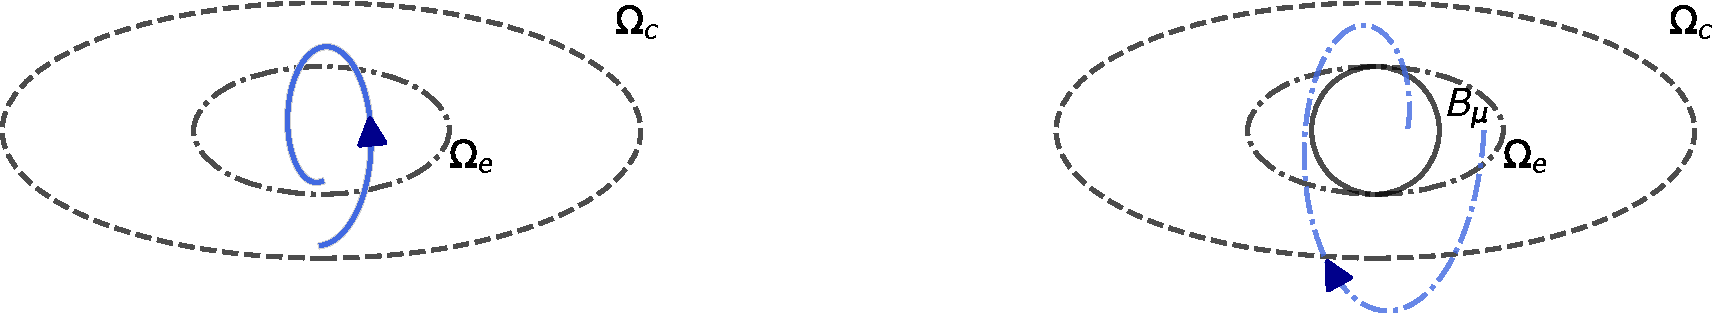
\includegraphics[width=\textwidth]{ultimate_boundedness_rotated.pdf}
		\caption{}
		\label{fig:boundedness_vs_ultimate_boundedness}
	\end{figure}
	\vspace{-2cm}
	\begin{columns}[t,totalwidth=\textwidth]
        \column{0.47\textwidth}
		\begin{tcolorbox}[title=Boundedness:]
			\vspace{-0.4cm}
			\begin{align*}
				\|\underline{x}(t_0)\| \leq \alpha \Rightarrow \|\underline{x}(t)\| \leq \beta,
				\\ c>0, \alpha\in(0,c),\, \beta>0,\,\forall\, t \geq t_0
			\end{align*}		
		\end{tcolorbox}
		
        \column{0.47\textwidth}
		\begin{tcolorbox}[title=Ultimate Boundedness:]
			\vspace{-0.4cm}
			\begin{align*}
				\|\underline{x}(t)\| \leq b 
				\\ \forall\, t \geq t_0+T
			\end{align*}
		\end{tcolorbox}
    \end{columns}
\end{frame}


%%%%%%%%%%%%%%%%%%%%%%%%%%%%%%%%%%%%%%%%%%%%%%%%%%%%%
\section{Vanishing Perturbations}

\begin{frame}
    \frametitle{Lyapunov Stability for Vanishing Perturbations}

    \textbf{Problem:} Analyze stability of $\dot{\underline{x}} = f(\underline{x}) + g(\underline{x}, t)$
    \begin{itemize}
        \item Nominal system ($\dot{\underline{x}} = f(\underline{x})$) exponentially stable
    \end{itemize}
	\vspace{0.3cm}
    \textbf{Assumptions for Exponential Stability:}
    \begin{itemize}
        \item Perturbation $g(\underline{x}, t)$ vanishes (i.e., $g(\underline{x}, t) \to 0$ as $\underline{x} \to 0$)
        \item $V(t,\underline{x})$: continuously differentiable, positive definite, radially unbounded
    \end{itemize}
    \vspace{0.3cm} % Reduced vertical space
    \textbf{Condition for Global Uniform Exponential Stability:}
    \begin{align*}
        \frac{\partial V}{\partial t}+\frac{\partial V}{\partial \underline{x}}f(\underline{x}) &\leq -c_3\|\underline{x}\|^2 \text{ and } \left\|\frac{\partial V}{\partial \underline{x}}\right\| \leq c_4\|\underline{x}\| \\[0.5em]
        \|g(\underline{x},t)\| &\leq \gamma\|\underline{x}\| \text{ where } 0 \leq \gamma(t) < \frac{c_3}{c_4}
    \end{align*}

\end{frame}

% \begin{frame}
%     \frametitle{Comparison Lemma - Example}

% 	\vspace{-0.5cm}
% 	\begin{tcolorbox}[title=Problem: Analyze stability of a scalar perturbed system]
% 		\vspace{-0.4cm}
% 		\begin{align*}
% 			\dot{\underline{x}} = -a\,\underline{x}(t) + g(t, \underline{x}), \quad \underline{x}(0) = 0, \quad a > 0
% 		\end{align*}
% 	\end{tcolorbox}

%     \textbf{Assumptions/Conditions:}
%     \begin{itemize}
%         \item $\underline{x}(t) \geq 0 \quad \forall\, t \geq 0$
%         \item $g(t, \underline{x}) \leq b\,\underline{x}(t) \quad \forall\, \underline{x} \geq 0$
%     \end{itemize}
% 	\vspace{0.3cm}
% 	\textbf{Integral Condition:}
% 	\begin{align*}
% 	\underline{x}(t) \leq \underline{x}_0 + \int_{t_0}^{t} \gamma(\tau)\, d\tau
% 	= \underline{x}_0 + \int_{t_0}^{t} [-a\,\underline{x}(\tau) + b\,\underline{x}(\tau)]\, d\tau
% 	\end{align*}
% 	\vspace{0.3cm}
% 	\textbf{Bound for Derivative:}
% 	\begin{align*}
% 	\dot{\underline{x}}(t) \leq -a\,\underline{x}(t) + b\,\underline{x}(t) = -(a - b)\,\underline{x}(t)
% 	\end{align*}
% 	\end{frame}
	
% \begin{frame}
% 	\frametitle{Comparison Lemma - Example}
% 	\textbf{From the Bound for Derivative:}
% 	\begin{align*}
% 		\underline{x}(t) \leq \underline{x}_0 + \int_{t_0}^{t} \dot{\underline{x}}(\tau)\, d\tau
% 		\leq \underline{x}_0 - (a - b) \int_{t_0}^{t} \underline{x}(\tau)\, d\tau
% 	\end{align*}
% 	\vspace{0.3cm}
% 	\textbf{Note:} This applies if $(a-b)\underline{x}$ is continuous, positive definite, and non-decreasing
% 	\vspace{-0.3cm}
% 	\begin{tcolorbox}[title=Conclusion: Exponential Stability of the Perturbed System]
% 		\vspace{-0.4cm}
% 		\begin{align*}
% 			\lim_{t \to \infty} \underline{x}(t) = 0 \\[0.3cm]
% 			\underline{x}(t) \leq \underline{x}_0\, e^{-(a - b)(t-t_0)}
% 		\end{align*}
% 	\end{tcolorbox}
% \end{frame}

% \begin{frame}
%     \frametitle{Comparison Lemma - Example}

%     \vspace{-0.5cm}
%     \begin{tcolorbox}[title=Problem: Analyze stability of a scalar perturbed system]
%         \vspace{-0.4cm}
%         \begin{align*}
%             \dot{\underline{x}} = -a\,\underline{x}(t) + g(t, \underline{x}), \quad \underline{x}(0) = \underline{x}_0, \quad a > 0
%         \end{align*}
%     \end{tcolorbox}

%     \textbf{Assumptions/Conditions:}
%     \begin{itemize}
%         \item $\underline{x}(t) \geq 0 \quad \forall\, t \geq 0$
%         \item $g(t, \underline{x}) \leq b\,\underline{x}(t) \quad \forall\, \underline{x} \geq 0$ and $0 \leq b < a$
%     \end{itemize}

%     \vspace{0.3cm}
%     \textbf{Step 1: Integral form of the solution}
%     \begin{align*}
%         \underline{x}(t) = \underline{x}(t_0) + \int_{t_0}^{t} \dot{\underline{x}}(\tau)\, d\tau
%     \end{align*}
%     \begin{align*}
%         \underline{x}(t) \leq \underline{x}(t_0) + \int_{t_0}^{t} \left[-a\,\underline{x}(\tau) + b\,\underline{x}(\tau)\right] d\tau = \underline{x}(t_0) - (a - b) \int_{t_0}^{t} \underline{x}(\tau)\, d\tau
%     \end{align*}
% \end{frame}

% \begin{frame}
%     \frametitle{Comparison Lemma - Example}

%     \textbf{Step 2: Define comparison function } $\underline{z}(t)$:
%     \begin{align*}
%         \underline{z}(t) = \underline{x}(t_0) - (a - b) \int_{t_0}^{t} \underline{z}(\tau)\, d\tau
%     \end{align*}
%     \begin{align*}
%         \dot{\underline{z}}(t) = -(a - b)\,\underline{z}(t), \quad \underline{z}(t_0) = \underline{x}(t_0)
%     \end{align*}

%     \textbf{Solution:}
%     \begin{align*}
%         \underline{z}(t) = \underline{x}(t_0)\, e^{-(a - b)(t - t_0)}
%     \end{align*}

%     \vspace{-0.3cm}
%     \begin{tcolorbox}[title=Conclusion: Exponential Stability of the Perturbed System]
%         \vspace{-0.4cm}
%         \begin{align*}
%             \lim_{t \to \infty} \underline{x}(t) = 0 \\[0.3cm]
%             \underline{x}(t) \leq \underline{x}(t_0)\, e^{-(a - b)(t - t_0)}
%         \end{align*}
%     \end{tcolorbox}
% \end{frame}

\begin{frame}
    \frametitle{Comparison Lemma - Example}

    \vspace{-0.5cm}
    \begin{tcolorbox}[title=Problem: Analyze stability of a scalar perturbed system]
        \vspace{-0.4cm}
        \begin{align*}
            \dot{\underline{x}}(t) = -a\,\underline{x}(t) + g(t, \underline{x}), \quad \underline{x}(t_0) = \underline{x}_0, \quad a > 0
        \end{align*}
    \end{tcolorbox}

    \textbf{Assumptions/Conditions:}
    \begin{itemize}
        \item $\underline{x}(t) \geq 0$ for all $t \geq t_0$
        \item $g(t, \underline{x})$ is bounded: $g(t, \underline{x}) \leq b\,\underline{x}(t) \quad \forall\, \underline{x} \geq 0$ and $0 \leq b < a$.
    \end{itemize}

    \vspace{0.3cm}
    \begin{columns}
        \column{0.48\textwidth}
        \textbf{Step 1: Formulate the comparison inequality}
        \begin{align*}
            \dot{\underline{x}}(t) &\leq -a\,\underline{x}(t) + b\,\underline{x}(t) \\[0.3cm]
            \dot{\underline{x}}(t) &\leq -(a - b)\,\underline{x}(t)
        \end{align*}

        \column{0.48\textwidth}
        \textbf{Step 2: Define a comparison system} \\
        \begin{align*}
            \dot{\underline{z}}(t) &= -(a - b)\,\underline{z}(t) \\[0.3cm]
            \underline{z}(t_0) &= \underline{x}(t_0)
        \end{align*}
    \end{columns}
    
\end{frame}

\begin{frame}
    \frametitle{Comparison Lemma - Example}
    \begin{columns}
        \column{0.48\textwidth}
        \textbf{Step 3: Solve the comparison system} \\
        \begin{align*}
            \underline{z}(t) = \underline{x}(t_0)\, e^{-(a - b)(t - t_0)}
        \end{align*}

        \column{0.48\textwidth}
        \textbf{Step 4: Apply the Comparison Lemma (Grönwall Inequality)}
        % Since $\dot{\underline{x}}(t) \leq -(a - b)\,\underline{x}(t)$ and $\dot{\underline{z}}(t) = -(a - b)\,\underline{z}(t)$, with $\underline{x}(t_0) = \underline{z}(t_0)$, the Comparison Lemma states that:
        \begin{align*}
            \underline{x}(t) \leq \underline{z}(t) \quad \forall\, t \geq t_0
        \end{align*}
    \end{columns}

    \vspace{0.3cm}
    \begin{tcolorbox}[title=Conclusion: Exponential Stability of the Perturbed System]
        \vspace{-0.4cm}
        % Given our assumption that $0 \leq b < a$, it follows that $(a - b) > 0$.
        % Therefore, the exponent $-(a - b)(t - t_0)$ is negative and decreases linearly with $t$.
        \begin{align*}
            \lim_{t \to \infty} e^{-(a - b)(t - t_0)} = \lim_{t \to \infty} \underline{x}(t) = 0
        \end{align*}
        \begin{align*}
            \underline{x}(t) \leq \underline{x}(t_0)\, e^{-(a - b)(t - t_0)}
        \end{align*}
    \end{tcolorbox}
\end{frame}

%%%%%%%%%%%%%%%%%%%%%%%%%%%%%%%%%%%%%%%%%%%%%%%%%%%%%
\section{Non-Vanishing Perturbations}

\begin{frame}
    \frametitle{Non-Vanishing Perturbations: The Problem}

    \textbf{Challenge:}
    \begin{itemize}
        \item Perturbation does not vanish $\Rightarrow$ exact convergence to zero is impossible
        \item State $\underline{x}(t)$ will always be pushed away from origin
    \end{itemize}

    \vspace{0.3cm}
    \textbf{Goal: Ultimate Boundedness}
    \begin{itemize}
        \item We seek boundedness around origin
        \item “Good enough” stability for real-world systems
    \end{itemize}

    \vspace{0.3cm}
    \textbf{Analogy:}
    \begin{itemize}
        \item Like balancing a pencil in wind as it won’t stay still
        \item We can bound how far it wobbles
    \end{itemize}
\end{frame}

\begin{frame}
    \frametitle{Lyapunov Conditions for Ultimate Boundedness}

    \textbf{System:} $\dot{\underline{x}} = f(\underline{x}) + g(\underline{x}, t)$
    \begin{itemize}
        \item Origin is exponentially stable for nominal system ($g \equiv 0$)
    \end{itemize}

    \vspace{0.3cm}
    \textbf{Lyapunov Function Conditions:}
    \begin{itemize}
        \item $V(\underline{x})$ positive definite, radially unbounded, continuously differentiable
        % \item \textit{Dummies: $V$ is like energy; positive means it's big away from origin, zero at origin.}
        \item $\dot{V} \leq -c_3\|\underline{x}\|^2$ for nominal dynamics
        % \item \textit{Dummies: How fast "energy" changes w.r.t. position; not too steep.}
        \item $\left\|\frac{\partial V}{\partial \underline{x}}\right\| \leq c_4\|\underline{x}\|$
    \end{itemize}

    \vspace{0.3cm}
    % \textit{Dummies: External disturbance is noisy but has a finite maximum strength $\delta$.}
    \textbf{Key Trade-off:}
    \[
        \|g(\underline{x}, t)\| \leq\delta < \frac{c_3}{c_4} \sqrt{\frac{c_1}{c_2}}\, \theta r, \quad \theta \in (0,1)
    \]
\end{frame}

\begin{frame}
    \frametitle{Result: Initial Decay and Ultimate Boundedness}

    \vspace{-0.4cm}
    \begin{tcolorbox}[title=For $\|\underline{x}(t_0)\| \leq \sqrt{c_1/c_2} \, r$]
        \textbf{Phase 1: Initial Exponential Decay} \quad ($t_0 \leq t \leq t_0 + T$)
        \begin{align*}
            \|\underline{x}(t)\| \leq k\, e^{-\gamma (t - t_0)} \|\underline{x}(t_0)\|
        \end{align*}
        \textbf{Phase 2: Ultimate Bound} \quad ($t \geq t_0 + T$)
        \begin{align*}
            \|\underline{x}(t)\| \leq b
        \end{align*}
    \end{tcolorbox}

    \vspace{0.2cm}
    \textbf{Interpretation:}
    \begin{itemize}
        \item System initially decays toward origin
        \item Perturbation prevents full convergence
        \item Final “wobble size” $b$ depends on $\delta$, $c_1$ – $c_4$
    \end{itemize}

    % \vspace{0.3cm}
    % \textbf{Key Parameters:}
    % \[ k = \sqrt{\frac{c_2}{c_1}}, \quad \gamma = \frac{(1 - \theta)c_3}{2c_2}, \quad b = \frac{c_4}{c_3}k \frac{\delta}{\theta} \]
    % \textit{Dummies: These are like calibration numbers telling us how fast it decays ($k, \gamma$) and how big the final wobble will be ($b$).}
\end{frame}


\begin{frame}
    \frametitle{Example: Bounded Disturbance Response}
	\vspace{-0.5cm}
    \begin{tcolorbox}[title=Problem: Analyze Boundedness of a Perturbed Mass-Spring-Damper-System]
		\vspace{-0.4cm}
        \begin{align*}
            \dot{x}_1 &= x_2 \\ % Position
            \dot{x}_2 &= -2x_1 - 3x_2 + d
        \end{align*}
        with bounded disturbance $|d| \leq \delta$ and the origin of the nominal system being exponentially stable
    \end{tcolorbox}

    \vspace{0.3cm}
    \textbf{Lyapunov Candidate Function:} $V(\underline{x}) = \underline{x}^T P \underline{x}$
    \begin{itemize}
        \item $P > 0$ found by solving $A^T P + P A = -Q$
        \vspace{0.2cm}
        \item For $Q>0$ and $A = \begin{bmatrix} 0 & 1 \\ -2 & -3 \end{bmatrix}$
        % \item $c_1 \|\underline{x}\|^2 \leq V(\underline{x}) \leq c_2 \|\underline{x}\|^2$
    \end{itemize}

\end{frame}

\begin{frame}
    \frametitle{Example: Bounded Disturbance Response}

    \textbf{Applying Lyapunov Stability Conditions:}
		\[ \dot{V} \leq -c_3 \|\underline{x}\|^2 + c_4 \|d\| \|\underline{x}\| \leq -c_3 \|\underline{x}\|^2 + c_4 \delta \|\underline{x}\| \]

    % \vspace{0.3cm}
    % \textbf{Recalling Boundedness Condition:}
    % \begin{itemize}
    %     \item If $\delta$ satisfies the condition:
    %           \[ \delta < \frac{c_3}{c_4} \sqrt{\frac{c_1}{c_2}} \theta r, \quad \theta \in (0,1), r>0 \]
    %           (This ensures the "pull towards zero" is stronger than the "push from disturbance" outside a small ball.)
    % \end{itemize}

    \vspace{-0.1cm}
    \begin{tcolorbox}[title=Conclusion: Ultimate Boundedness Guaranteed]
        \begin{itemize}
            \item System state $\|\underline{x}(t)\|$ eventually converges to and remains within a bounded region:
                  \[ \|\underline{x}(t)\| \leq b \quad \forall\, t \geq t_0 + T \]
            \item The ultimate bound $b$ and other parameters are:
                  \[ b = \frac{c_4}{c_3} k \frac{\delta}{\theta}, \quad k = \sqrt{c_2/c_1} \]
            \item Size of the ultimate bound $b$ directly \textbf{scales with the disturbance magnitude $\delta$}
        \end{itemize}
    \end{tcolorbox}
\end{frame}


%%%%%%%%%%%%%%%%%%%%%%%%%%%%%%%%%%%%%%%%%%%%%%%%%%
\section{Summary and Discussion}

\begin{frame}
    \frametitle{Key Insights \& Practical Implications}

    \textbf{Theoretical Insights:}
    \begin{itemize}
        \setlength{\itemsep}{8pt}
        \item Lyapunov methods: unify time-varying and perturbed system analysis
        \item Perturbation type: dictates achievable stability properties
        \item Ultimate boundedness: models real-world robustness
    \end{itemize}

    \vspace{0.8cm}
    \textbf{Design Implications:}
    \begin{itemize}
        \setlength{\itemsep}{8pt}
        \item Small, vanishing perturbations: maintains exponential convergence
        \item Persistent disturbances: design for bounded operation
        \item Robustness: requires accurate perturbation characterization
    \end{itemize}
\end{frame}




%%%%%%%%%%%%%%%%%%%%%%%%%%%%%%%%%%%%%%%%%%%%%%%%%%%%%
\appendix

\begin{frame}[allowframebreaks]
    \frametitle{References}
    \nocite{*} 
    \printbibliography[heading=none]
\end{frame}

\end{document}
